\clearpage
\section{电动轮椅(Mmechatronic drive module) 框图建模}

%%%%%%%%%%%%%%%%%
\begin{figure*}[h]
	\centering
	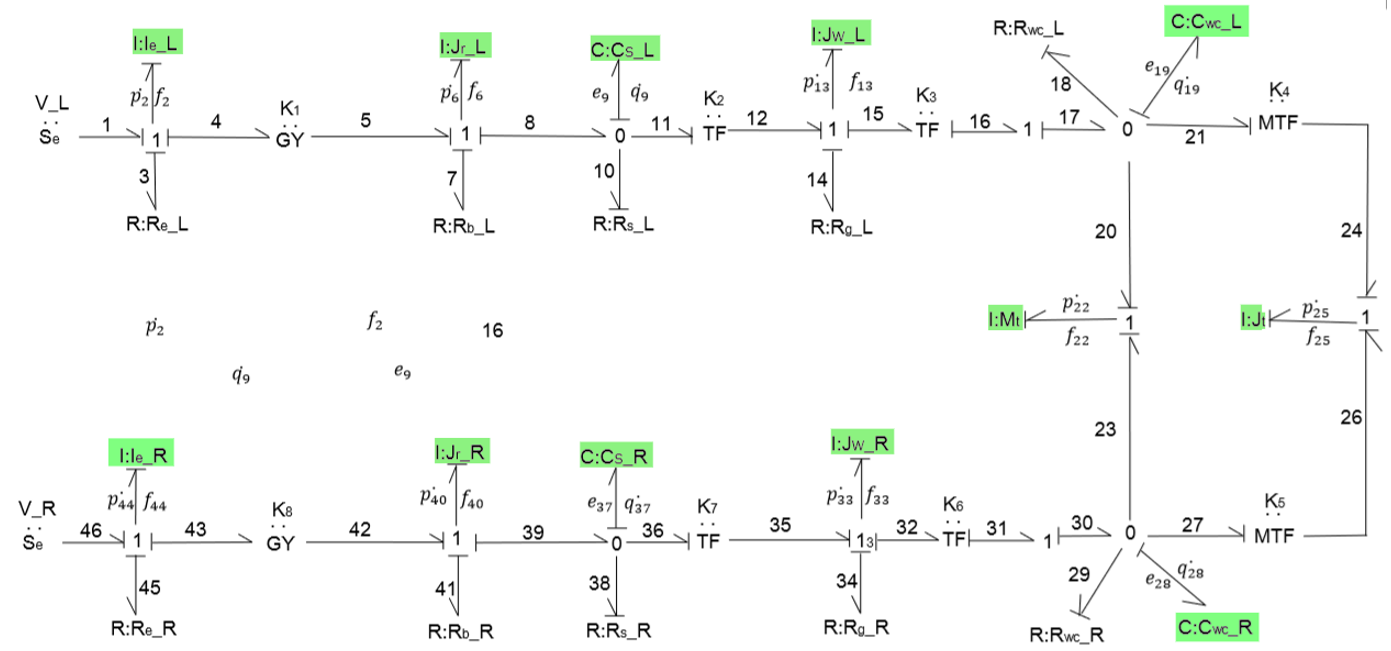
\includegraphics[width=\textwidth]{fig/MDM.png}
	\caption{MDM因果化标注。}\label{fig:mdm}
\end{figure*}
%%%%%%%%%%%%%%%%%
\subsection{状态空间方程推导}
\subsubsection{状态变量$\dot{ p_2 }$}
%%%%%%%%%%%%%%%%%
\begin{figure*}[h]
	\centering
	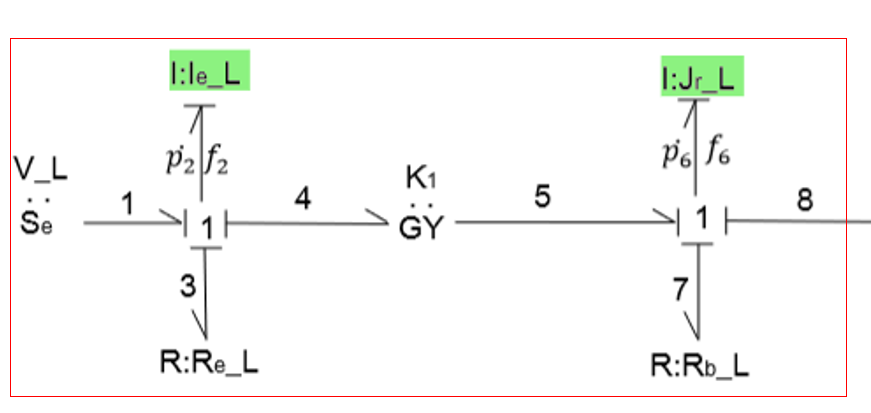
\includegraphics[width=0.5\textwidth]{fig/equation1.png}
	\caption{}\label{fig:equation1}
\end{figure*}
%%%%%%%%%%%%%%%%%
对于$\dot{p} _ { 2 }$,开始列写方程,利用键合图的因果关系求出$e_2$:根据功率流方向标注,势变量$e_2$来自1结的输出,是由$e_1$,$e_3$,和$e_4$产生的,因此:
\begin{equation}\label{p2}
\dot{p} _ { 2 } = e _ { 2 } = e _ { 1 } - e _ { 3 } - e _ { 4 },
\end{equation}
$e_1$是输入变量,一直保留在最终的方程中;$e_3$来自阻性元件$R _ { eL }$的输出;$e_4$直接与状态变量有关,故而有下面三式:
\begin{equation}\label{e1}
e _ { 1} = V_L,
\end{equation}
\begin{equation}\label{e3}
e _ { 3 } = f _ { 3 } R _ { eL  }  = f _ { 2 } R _ { eL }  = \frac { p _ { 2 } } { I _ { eL } } R _ { eL},
\end{equation}
\begin{equation}\label{e4}
e _ { 4 } = k _ { 1 } f _ { 5 } = k _ { 1 } f _ { 6 } = k _ { 1 } \frac { p _ { 6 } } { J _ { r L}  },
\end{equation}
由式(\ref{p2})-(\ref{e4})得到状态方程1:
\begin{equation}
\dot { p } _ { 2 } = V _ {L}  - \frac { p _ { 2 } } { I _ { eL}  } R _ { eL} - k _ { 1 } \frac { p _ { 6 } } { J _ { rL} },
\end{equation}

%%%%%%%%%%%%%%%%%%%%%%%%%%%%%%%%%%%%%%%%%%%%%%%%%%%%%%%%%%%%%%%%
%%%%%%%%%%%%%%%%%%%%%%%%%%%%%%%%%%%%%%%%%%%%%%%%%%%%%%%%%%%%%%%%
%%%%%%%%%%%%%%%%%%%%%%%%%%%%%%%%%%%%%%%%%%%%%%%%%%%%%%%%%%%%%%%%
\subsubsection{状态变量$\dot{ p_6 }$}
%%%%%%%%%%%%%%%%%
\begin{figure}[H]
	\centering
	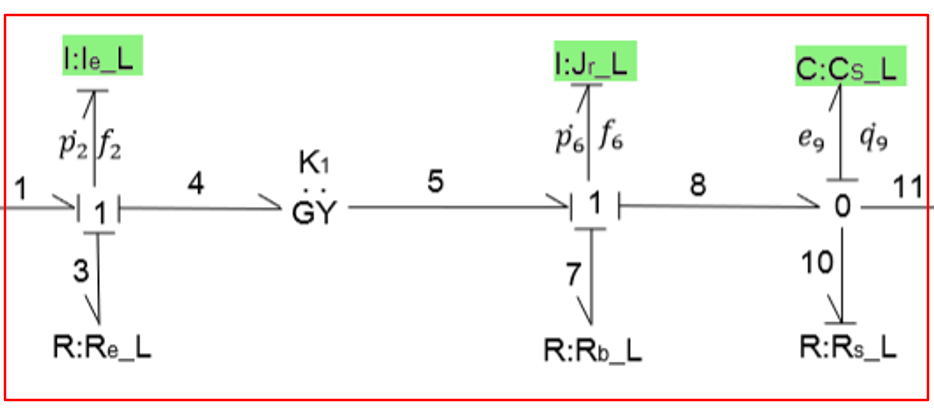
\includegraphics[width=0.5\textwidth]{fig/equation2.png}
	\caption{}\label{fig:equation2}
\end{figure}
%%%%%%%%%%%%%%%%%
对于$\dot{p} _ { 6 }$,开始列写方程,利用键合图的因果关系求出$e_6$:根据功率流方向标注,势变量$e_6$来自1结的输出,是由$e_5$,$e_7$,和$e_8$产生的,因此:
\begin{equation}\label{p6}
\dot{ p } _ { 6 } = e _ { 6 } = e _ { 5 } - e _ { 7 } - e _ { 8 },
\end{equation}
$e_5$直接与状态变量有关;$e_7$来自阻性元件$R _ { bL }$的输出;$e_8$同样直接与状态变量有关,故而有下面三式:
\begin{equation}
e _ { 5 } = k _ { 1 } f _ { 4 } = k _ { 1 } f _ { 2 } = k _ { 1 } \frac { p _ { 2 } } { I _ { eL }  },
\end{equation}
\begin{equation}
e _ { 7 } = f _ { 7 } R _ { bL }  = f _ { 6 } R _ { b L }  = \frac { p _ { 6 } } { J _ { rL }  } R _ { bL} ,
\end{equation}

\begin{equation}\label{e8}
e _ { 8 } = e _ { 9 } = \frac { q _ { 9 } } { C _ { s L}  } ,
\end{equation}
由式\ref{p6}-\ref{e8}得到状态方程2:
\begin{equation}
\dot{ p } _ { 6 } = k _ { 1 } \frac { p _ { 2 } } { I _ { e L }  } - \frac { p_ { 6 } } { J _ { rL}  } R _ { bL}  - \frac { q _ { 9 } } { C _ { sL }  }.
\end{equation}
%%%%%%%%%%%%%%%%%%%%%%%%%%%%%%%%%%%%%%%%%%%%%%%%%%%%%%%%%%%%%%%%
%%%%%%%%%%%%%%%%%%%%%%%%%%%%%%%%%%%%%%%%%%%%%%%%%%%%%%%%%%%%%%%%
%%%%%%%%%%%%%%%%%%%%%%%%%%%%%%%%%%%%%%%%%%%%%%%%%%%%%%%%%%%%%%%%
\subsubsection{状态变量$\dot{ q_9 }$}
%%%%%%%%%%%%%%%%%
\begin{figure*}[h]
	\centering
	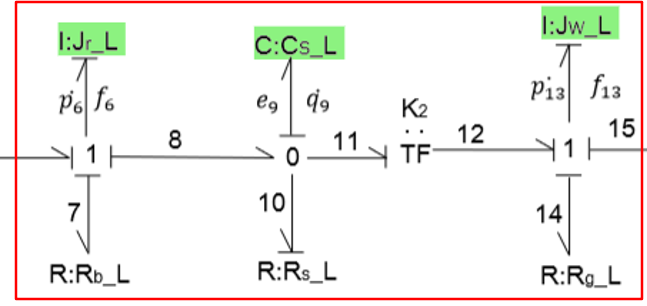
\includegraphics[width=0.5\textwidth]{fig/equation3.png}
	\caption{}\label{fig:equation3}
\end{figure*}
%%%%%%%%%%%%%%%%%
对于$\dot{q} _ { 9 }$,开始列写方程,通过使用因果关系对$f_9$路径进行跟踪,流变量$f_9$是对$C_{sL}$的输入,从0结出来的输出,此输出由因果输入$f _ { 8 }$, $ f _ { 10 }$, $  f _ { 11 }$产生,因此:
\begin{equation}\label{q9}
\dot{ q }_{ 9 } = f _ { 9 } = f _ { 8 } - f _ { 10 } - f _ { 11 },
\end{equation}
$f_8$直接与状态变量有关;$f_{10}$来自阻性元件$R _ { sL }$的输出;$f_{11}$同样直接与状态变量有关,故而有下面三式:
\begin{equation}
f _ { 8 } = f _ { 6 } = \frac { p _ { 6 } } { J _ { r L } },
\end{equation}
\begin{equation}
f _ { 10 } = \frac { e _ { 10 } } { R _ { sL}  } = \frac { e _ { 9 } } { R _ { sL }  } = \frac { q _ { 9 } } { C _ { s L}  R _ { s  L } } ,
\end{equation}

\begin{equation}\label{f11}
f _ { 11 } = \frac { f _ { 12 } } { k _ { 2 } } = \frac { f _ { 13 } } { k _ { 2 } } = \frac { p _ { 13 } } { J _ { wL}  k _ { 2 } },
\end{equation}
由式\ref{q9}-\ref{f11}得到状态方程3:
\begin{equation}
\dot{ q } _ { 9 } = \frac { p _ { 6 } } { J _ { rL } } - \frac { q _ { 9 } } { C _ { sL }  R _ { s L}  } - \frac { p _ { 13 } } { J _ { w L }  k _ { 2 } }.
\end{equation}
%%%%%%%%%%%%%%%%%%%%%%%%%%%%%%%%%%%%%%%%%%%%%%%%%%%%%%%%%%%%%%%%
%%%%%%%%%%%%%%%%%%%%%%%%%%%%%%%%%%%%%%%%%%%%%%%%%%%%%%%%%%%%%%%%
%%%%%%%%%%%%%%%%%%%%%%%%%%%%%%%%%%%%%%%%%%%%%%%%%%%%%%%%%%%%%%%%
\subsubsection{状态变量$\dot{ p}_{13} $}
%%%%%%%%%%%%%%%%%
\begin{figure}[H]
	\centering
	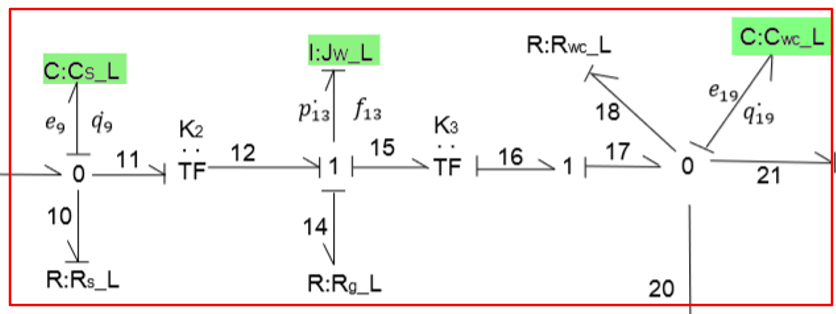
\includegraphics[width=0.5\textwidth]{fig/equation4.png}
	\caption{}\label{fig:equation4}
\end{figure}
%%%%%%%%%%%%%%%%%
对于$\dot{p} _ { 13 }$,开始列写方程,利用键合图的因果关系求出$e_{13}$:根据功率流方向标注,势变量$e_{13}$来自1结的输出,是由$e_{12}$,$e_{14}$,和$e_{15}$产生的,因此:
\begin{equation}\label{p13}
\dot{ p } _ { 13 } = e _ { 12 } - e _ { 14 } - e _ { 15 },
\end{equation}
$e_{12}$直接与状态变量有关;$e_{14}$来自阻性元件$R _ { gL }$的输出;$e_{15}$同样直接与状态变量有关,故而有下面三式:
\begin{equation}
e _ { 12 } = \frac { e _ { 11 } } { k _ { 2 } } = \frac { e _ { 9 } } { k _ { 2 } } = \frac { q _ { 9 } } { C _ { sL  } k _ { 2 } },
\end{equation}
\begin{equation}
e _ { 14 } = f _ { 14 } R _ { gL}  = f _ { 13 } R _ { gL}  = \frac { p _ { 13 } } { J _ { wL}  } R _ { gL } ,
\end{equation}

\begin{equation}\label{e15}
e _ { 15 } = e _ { 16 } k _ { 3 } = e _ { 17 } k _ { 3 } = e _ { 19 } k _ { 3 } = \frac { q _ { 19 } } { C _ { w cL }  } k _ { 3 } ,
\end{equation}
由式\ref{p13}-\ref{e15}得到状态方程4:
\begin{equation}
\dot{ p }_ { 13 } = \frac { q _ { 9 } } { C _ { sL}  k _ { 2 } } - \frac { p _ { 13 } } { J _ { wL}  } R _ { gL }  - \frac { q _ { 19 } } { C _ { w cL}  } k _ { 3 }.
\end{equation}
%%%%%%%%%%%%%%%%%%%%%%%%%%%%%%%%%%%%%%%%%%%%%%%%%%%%%%%%%%%%%%%%
%%%%%%%%%%%%%%%%%%%%%%%%%%%%%%%%%%%%%%%%%%%%%%%%%%%%%%%%%%%%%%%%
%%%%%%%%%%%%%%%%%%%%%%%%%%%%%%%%%%%%%%%%%%%%%%%%%%%%%%%%%%%%%%%%
\subsubsection{状态变量$\dot{ q}_{19}$}
%%%%%%%%%%%%%%%%%
\begin{figure*}[h]
	\centering
	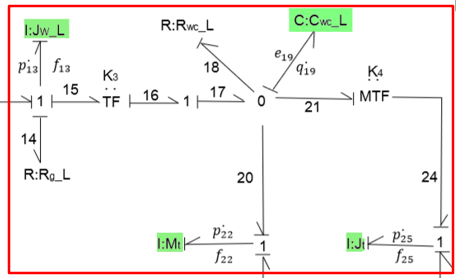
\includegraphics[width=0.5\textwidth]{fig/equation5.png}
	\caption{}\label{fig:equation5}
\end{figure*}
%%%%%%%%%%%%%%%%%
对于$\dot{q} _ { 19 }$,开始列写方程,通过使用因果关系对$f_{19}$路径进行跟踪,流变量$f_{19}$是对$C_{wcL}$的输入,从0结出来的输出,此输出由因果输入$f _ { 17 }$, $f _ { 18 }$, $ f _ { 20 }$, $  f _ { 21 }$产生,因此:
\begin{equation}\label{q19}
\dot { q } _ { 19 } = f _ { 17 } - f _ { 18 } - f _ { 20 } - f _ { 21 },
\end{equation}
$f_{17}$直接与状态变量有关;$f_{18}$来自阻性元件$R _ { wcL }$的输出;$f_{20}$和$f_{21}$同样直接与状态变量有关,故而有下面四式:
\begin{equation}
f _ { 17 } = f _ { 16 } = f _ { 15 } k _ { 3 } = f _ { 13 } k _ { 3 } = \frac { p _ { 13 } } { J _ { w L} } k _ { 3 },
\end{equation}
\begin{equation}
f _ { 18 } = \frac { e _ { 18 } } { R _ { w c L}  } = \frac { e _ { 19 } } { R _ { w cL  } } = \frac { q _ { 19 } } { C _ { w c  L} R _ { w c L } },
\end{equation}
\begin{equation}
f _ { 20 } = f _ { 22 } = \frac { p _ { 22 } } { M _ { t } },
\end{equation}
\begin{equation}\label{f21}
f _ { 21 } = \frac { f _ { 24 } } { k _ { 4 } } = \frac { f _ { 25 } } { k _ { 4 } } = \frac { p _ { 25 } } { J _ { t } k _ { 4 } },
\end{equation}
由式\ref{q19}-\ref{f21}得到状态方程5:
\begin{equation}
\dot { q } _ { 19 } = \frac { p _ { 13 } } { J _ { w L }  } k _ { 3 } - \frac { q _ { 19 } } { C _ { w c L }  R _ { w c L }  } - \frac { p _ { 22 } } { M _ { t } } - \frac { p _ { 25 } } { J _ { t } k _ { 4 } }.
\end{equation}
%%%%%%%%%%%%%%%%%%%%%%%%%%%%%%%%%%%%%%%%%%%%%%%%%%%%%%%%%%%%%%%%
%%%%%%%%%%%%%%%%%%%%%%%%%%%%%%%%%%%%%%%%%%%%%%%%%%%%%%%%%%%%%%%%
%%%%%%%%%%%%%%%%%%%%%%%%%%%%%%%%%%%%%%%%%%%%%%%%%%%%%%%%%%%%%%%%
\subsubsection{状态变量$\dot{ p}_{22} $}
%%%%%%%%%%%%%%%%%
\begin{figure}[H]
	\centering
	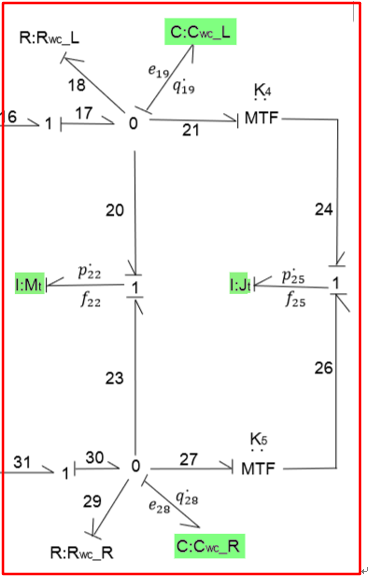
\includegraphics[width=0.25\textwidth]{fig/equation6.png}
	\caption{}\label{fig:equation6}
\end{figure}
%%%%%%%%%%%%%%%%%
对于$\dot{p} _ { 22 }$,开始列写方程,利用键合图的因果关系求出$e_{22}$:根据功率流方向标注,势变量$e_{22}$来自1结的输出,是由$e_{20}$和$e_{23}$产生的,因此:
\begin{equation}\label{p22}
\dot{ p }  _ { 22 } = e _ { 22 } = e _ { 20 } + e _ { 23 },
\end{equation}
$e_{20}$与$e_{23}$均直接与状态变量有关,故而有下面两式:
\begin{equation}
e _ { 20 } = e _ { 19 } = \frac { q _ { 19 } } { C _ { w cL }  },
\end{equation}

\begin{equation}\label{e23}
e _ { 23 } = e _ { 28 } = \frac { q _ { 28 } } { C _ { w c R }  },
\end{equation}
由式\ref{p22}-\ref{e23}得到状态方程6:
\begin{equation}
\dot{ p } _ { 22 } = \frac { q _ { 19 } } { C _ { w c L } } + \frac { q _ { 28 } } { C _ { w c R  } }.
\end{equation}
%%%%%%%%%%%%%%%%%%%%%%%%%%%%%%%%%%%%%%%%%%%%%%%%%%%%%%%%%%%%%%%%
%%%%%%%%%%%%%%%%%%%%%%%%%%%%%%%%%%%%%%%%%%%%%%%%%%%%%%%%%%%%%%%%
%%%%%%%%%%%%%%%%%%%%%%%%%%%%%%%%%%%%%%%%%%%%%%%%%%%%%%%%%%%%%%%%
\subsubsection{状态变量$\dot{ p}_{25} $}
%%%%%%%%%%%%%%%%%
\begin{figure}[H]
	\centering
	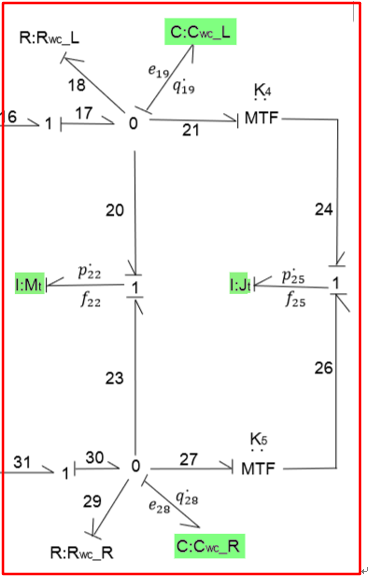
\includegraphics[width=0.25\textwidth]{fig/equation6.png}
	\caption{}\label{fig:equation6}
\end{figure}
%%%%%%%%%%%%%%%%%
对于$\dot{p} _ { 25 }$,开始列写方程,利用键合图的因果关系求出$e_{25}$:根据功率流方向标注,势变量$e_{22}$来自1结的输出,是由$e_{24}$和$e_{26}$产生的,因此:
\begin{equation}\label{p25}
\dot{ p } _ { 25 } = e _ { 24 } + e _ { 26 },
\end{equation}
$e_{24}$与$e_{26}$均直接与状态变量有关,故而有下面两式:
\begin{equation}
e _ { 24 } = \frac { e _ { 21 } } { k _ { 4 } } = \frac { e _ { 19 } } { k _ { 4 } } = \frac { q _ { 19 } } { C _ { w cL}  k _ { 4 } },
\end{equation}

\begin{equation}\label{e26}
e _ { 26 } = \frac { e _ { 27 } } { k _ { 5 } } = \frac { e _ { 28 } } { k _ { 5 } } = \frac { q _ { 28 } } { C _ { w c L }  k _ { 5 } },
\end{equation}
由式\ref{p25}-\ref{e26}得到状态方程7:
\begin{equation}
\dot{ p } _ { 25 } = \frac { q _ { 19 } } { C _ { w c L}  k _ { 4 } } + \frac { q _ { 28 } } { C _ { w cL }  k _ { 5 } }.
\end{equation}
%%%%%%%%%%%%%%%%%%%%%%%%%%%%%%%%%%%%%%%%%%%%%%%%%%%%%%%%%%%%%%%%
%%%%%%%%%%%%%%%%%%%%%%%%%%%%%%%%%%%%%%%%%%%%%%%%%%%%%%%%%%%%%%%%
%%%%%%%%%%%%%%%%%%%%%%%%%%%%%%%%%%%%%%%%%%%%%%%%%%%%%%%%%%%%%%%%
\subsubsection{根据对称性得到剩余状态方程}
根据对称性,另外五个状态方程见\ref{q28}-\ref{p44}:
\begin{equation}\label{q28}
\dot{ q}  _ { 28 } = \frac { p _ { 33 } } { J _ { w R }  } k _ { 6 } - \frac { q _ { 28 } } { C _ { w cR }  R _ { w c R } } - \frac { p _ { 22 } } { M _ { t } } - \frac { p _ { 25 } } { J _ { t } k _ { 5 } }.
\end{equation}
\begin{equation}
\dot{ p } _ { 33 } = \frac { q _ { 37 } } { C _ { s R }  k _ { 7 } } - \frac { p _ { 33 } } { J _ { wR }  } R _ { gR }  - \frac { q _ { 28 } } { C _ { w cR }  } k _ { 6 }
\end{equation}
\begin{equation}
\dot{q} _ { 37 } = \frac { p _ { 40 } } { J _ { r R } } - \frac { q _ { 37 } } { C _ { sR }  R _ { sR}  } - \frac { p _ { 33 } } { J _ { w R}  k _ { 7 } }
\end{equation}
\begin{equation}
\dot{ p } _ { 40 } = k _ { 8 } \frac { p _ { 44 } } { I _ { e R}  } - \frac { p _ { 40 } } { J _ { r R }  } R _ { b R }  - \frac { q _ { 37 } } { C _ { s R } }
\end{equation}
\begin{equation}\label{p44}
\dot{ p } _ { 44 } = V _ {R}  - \frac { p _ { 44 } } { I _ { e R} } R _ { e R }  - k _ { 8 } \frac { p _ { 40 } } { J _ { r R  } }
\end{equation}
\subsection{键合图转框图}

\subsection{仿真结果}

可以将对象的工况分为两种情况:

\begin{enumerate}
	\item 在平坦路面上条件下,由人产生推力使轮椅向前运动。
	在该条件下,系统底部受到的速度输入较小且较不稳定。主要考虑以下几个参数:
	\begin{itemize}
		\item 车轮转动惯量,转动惯量;
		
		\item 车轮辐条刚度:存在于从车轮中心到地面由于充气轮胎所带来的弹簧/阻尼;
		
		\item 摩擦损失:存在于后充气轮和前脚轮与地面之间的阻力;
		
		\item 质量:包括椅子的重量和使用者的假定质量。该点位于重心处,获得系统平均质量。在降低模型的复杂性时,假设重心与后轮轴线中心重合。
	\end{itemize}
	
	\item 在平坦路面上条件下,由机电驱动模块产生使轮椅向前运动的动力。
	在该条件下,系统底部受到的速度输入较大且较稳定。主要考虑以下几个参数:
	\begin{itemize}
		\item 直流电动机的基本原理(包括电感,输出扭矩等)和基本性质(包括质量,电压等)。
		
		\item 传动部件的刚度,质量以及机械损失。
		
		\item 电动轮的转动惯量。
	\end{itemize}
	
\end{enumerate}



针对上述工况,结合简化模型的角度出发,做出如下假设:

\begin{itemize}
	
	\item 假设机械各部分零件为刚体;
	
	\item 假设刚体质心位于几何中心;
	
	\item 忽略铰接点连接处的摩擦;
	
	\item 忽略电驱动系统工作产热带来的参数变化。
	
\end{itemize}
